% SPDX-License-Identifier: CC-BY-4.0
% Copyright (c) 2026 Jonathan Yantis. Research draft; not submitted.
\documentclass[11pt,letterpaper]{article}
\usepackage[margin=0.85in]{geometry}
\usepackage[T1]{fontenc}
\usepackage{mathptmx,amsmath,amssymb,booktabs,array,ragged2e,xcolor,microtype,xurl,hyperref,fancyhdr,longtable,tikz}
\usetikzlibrary{arrows.meta,positioning}
\definecolor{studyblue}{RGB}{39,83,109}
\hypersetup{colorlinks=true,urlcolor=studyblue,citecolor=studyblue,linkcolor=black,pdfauthor={Jonathan Yantis},pdftitle={A Shared Time Base for Robotic gPTP and TSN Systems: PToB Edge Adaptation, Compatibility Boundaries, and a Validation Programme}}
\setlength{\parindent}{1em}\setlength{\parskip}{3pt}\setlength{\headheight}{14pt}\setlength{\emergencystretch}{2em}
\widowpenalty=10000\clubpenalty=10000
\renewcommand{\floatpagefraction}{0.8}\renewcommand{\topfraction}{0.9}\renewcommand{\textfraction}{0.1}
\pagestyle{fancy}\fancyhf{}\fancyhead[L]{\small PToB, gPTP and Robotics}\fancyhead[R]{\small Research draft, 22 October 2026}\fancyfoot[C]{\small\thepage}
\newcolumntype{L}[1]{>{\RaggedRight\arraybackslash}p{#1}}
\newcommand{\ns}{\,\mathrm{ns}}\newcommand{\us}{\,\mu\mathrm{s}}\newcommand{\ms}{\,\mathrm{ms}}\newcommand{\ppm}{\,\mathrm{ppm}}
\newcommand{\code}[1]{\texttt{#1}}
\begin{document}
\title{\vspace{-1.2em}A Shared Time Base for\\Robotic gPTP and TSN Systems\\[5pt]\large PToB Edge Adaptation, Compatibility Boundaries,\\and a Validation Programme}
\author{Jonathan Yantis}
\date{22 October 2026\\\small Research draft; not submitted or peer reviewed}
\maketitle
\begin{abstract}
A robot can synchronize its Ethernet clocks and still mislabel a camera exposure, miss a control deadline, or lose the temporal relationship to a wireless instrument. This paper investigates Precision Time over BLE (PToB) as a prospective timing extension at the edge of generalized Precision Time Protocol (gPTP) and Time-Sensitive Networking (TSN) systems. The proposed starting architecture follows an existing Ethernet time authority through a hardware-associated cross-clock map, distributes source-scoped time to BLE endpoints, and returns acquisition timestamps with explicit uncertainty and expiry. Ethernet traffic scheduling, application execution and physical actuation remain separately qualified services. A dated primary-source review distinguishes IEEE 802.1AS-2025, the published IEC/IEEE 60802-2026 industrial profile, Linux PTP, ROS 2 clock semantics and device-specific IEEE 1588 interfaces. We propose a domain, ancestry, event and quality contract; derive causal map composition, motion-error, holdover and schedule-margin constraints; and define independent validation gates with complete opportunity accounting. Historical PToB relative-phase observations motivate the research without establishing gPTP interoperability, TSN conformance or robot-output accuracy. BLE-derived time serving a new Ethernet island is a later, separately admitted mode; transparent carriage of gPTP across BLE is not claimed. No firmware change, new hardware measurement or operational robotics qualification accompanies this manuscript.
\end{abstract}
\noindent\small Copyright \copyright\ 2026 Jonathan Yantis. Original manuscript and figures: \href{https://creativecommons.org/licenses/by/4.0/}{CC BY 4.0}. Executable verification code: MIT.\normalsize

\section{Introduction}
A mobile manipulator may combine an Ethernet controller, joint drives, cameras, a lidar, a removable tool and a battery-powered inertial instrument. The wired devices may participate in a managed timing domain while the tool or instrument timestamps against a free-running local oscillator. A fusion pipeline then receives plausible timestamps whose origins, acquisition delays and validity differ. Replacing a callback timestamp with a better shared clock is useful, but only if that clock actually describes the sensor event and its relationship to the robot's time authority is known.

PToB studies shared time over Bluetooth Low Energy periodic advertising using source ancestry, causal clock maps and finite source validity \cite{viability}. These mechanisms suggest a focused adaptation: extend a named robot time domain to endpoints that need common event time but do not require an Ethernet interface. This is analogous to using a shared time base beneath media-specific adapters \cite{timecode}; the robotics boundary adds gPTP domains, hardware clocks, dynamic tools, scheduling deadlines and application-specific consequences of stale time.

Our hypothesis is conditional. A qualified Ethernet-to-PToB clock bridge could make wireless acquisition timestamps comparable with wired robot events while leaving the wired control network responsible for scheduled traffic. A later bridge could source an isolated Ethernet research island from PToB, provided it independently satisfies the chosen timing profile and source-quality policy. Neither route follows merely from emitting PTP-shaped packets or obtaining a small local clock-fit residual.

The contributions are (i) a dated primary-source compatibility review; (ii) a proposed source, domain, event and quality contract; (iii) explicit analytical budgets for clock transfer, moving sensors and schedules; and (iv) a staged programme that can reject the proposed adaptation. Literature was accessed on 22 October 2026. The latest discussed physical collection is the separate 22 October S3 study. Existing evidence remains historical and population-specific. This paper proposes an architecture and research plan, not a new normative wire profile or a demonstrated robot installation.

\section{Which robotics requirements need a common clock?}
\subsection{Four services with different acceptance criteria}
\emph{Event-time agreement} places an identified acquisition or observation on a shared coordinate. \emph{Frequency and phase control} makes physical oscillators or sampling edges track that coordinate. \emph{Bounded communication} delivers data within a stated deadline under an admitted traffic/topology envelope. \emph{Bounded execution and actuation} places a computation or physical output within its required interval. Clock synchronization can support all four; it does not establish the other three by itself.

The distinction appears in robotics literature. San Vicente Guti\'errez et al. report sub-microsecond clock synchronization, ROS 2 publication timestamping below $100\us$, and approximately 1--2 ms communication latency in their particular modular-robot setup \cite{modular}. Their measurements timestamp before publication and at subscription callback entry; those endpoints do not independently measure joint motion or sensor exposure. Their separate TSN study evaluates Ethernet shaping under competing traffic \cite{robottsn}. These are useful examples of different timing layers, not current ROS performance guarantees or a BLE comparison.

Table~\ref{tab:uses} separates candidate PToB services by their physical endpoint. The numerical requirements in this manuscript are explicit analytical examples, not universal robotics specifications. A deployment derives its limits from sensor dynamics, controller analysis, device capabilities and its applicable assurance process.

\begin{table}[htbp]\centering\small
\caption{Candidate robotics services. Every PToB adaptation here is proposed and unqualified.}\label{tab:uses}
\begin{tabular}{@{}L{0.22\linewidth}L{0.36\linewidth}L{0.35\linewidth}@{}}\toprule
Use case & Useful shared-time service & Additional acceptance boundary\\\midrule
Wireless IMU or tool sensor & Timestamp the actual sampling aperture or data-ready event; preserve sequence and source age. & Sensor pipeline delay, oscillator behavior and timestamp attachment must be measured.\\\addlinespace
Camera/lidar fusion & Relate exposure or per-point acquisition to wired encoder events. & Exposure/readout model, scan position and motion compensation; packet arrival is insufficient.\\\addlinespace
Instrumented gripper or removable tool & Bind contact/force events to robot state through docking and replacement. & Tool identity, counter reset, calibration scope and reacquisition interval.\\\addlinespace
Cross-robot experiment logging & Associate events across separately managed robot domains. & Explicit inter-domain relationship; no assumption of common epoch or independent references.\\\addlinespace
Scheduled joint actuation & Potential future common execution coordinate. & Qualified oscillator/output control, bounded transport and execution, and independent actuation evidence. Deferred beyond the initial sensor pilot.\\\bottomrule
\end{tabular}
\end{table}

\subsection{Timing error becomes a spatial error}
For a constant translational speed $v$, a timestamp error $\delta t$ contributes approximately $|\delta x|=|v\delta t|$. Under a bounded acceleration $a_{\max}$ over that interval, a conservative local estimate is
\begin{equation}
 E_x \leq v_{\max}E_t+\tfrac12 a_{\max}E_t^2,
 \qquad E_\theta\leq\omega_{\max}E_t,
 \label{eq:motion}
\end{equation}
where the angular expression assumes a bounded angular speed. These are temporal contributions only; extrinsic calibration, sensor noise, rolling shutter, deformation and estimator error remain additional terms.

At an assumed $2\,\mathrm{m/s}$, $100\us$ contributes $0.2\,\mathrm{mm}$ and $1\ms$ contributes $2\,\mathrm{mm}$ at constant speed. At an assumed $180^\circ/\mathrm{s}$, $100\us$ contributes $0.018^\circ$; at a one-metre lever arm its small-angle transverse contribution is approximately $0.314\,\mathrm{mm}$. A $10\us$ clock objective therefore cannot rescue an uncharacterized $1\ms$ acquisition delay. Conversely, some logging tasks can tolerate much more timing error than a coordinated sampling experiment.

\section{Documented standards and interface boundaries}\label{sec:survey}
\subsection{Survey method and version discipline}
We inspected standards-organization scope/status pages, official software documentation and source definitions, manufacturer documentation, and two original robotics papers. This selected survey establishes documented mechanisms and implementation questions. It is not a clause-by-clause conformance audit: the full normative texts of IEEE 802.1AS-2025 and IEC/IEEE 60802-2026 were not inspected. A future profile implementation must obtain the applicable editions and amendments and produce a requirement-to-evidence matrix.

IEEE identifies 802.1AS-2025 as an active standard, published 17 December 2025 and superseding 802.1AS-2020; its scope includes timing transport, source selection and indication of timing impairments \cite{as2025}. The industrial automation project lists IEC/IEEE 60802-2026 as published on 29 June 2026 \cite{industrial}. Calling 60802 merely a future draft would therefore misstate the status at this paper's access date. The profile selects features and configurations for industrial networks; it is not evidence that an arbitrary robot, Linux installation or BLE bridge conforms. The chosen base standard, amendments, media and domain configuration must be pinned together.

\subsection{Timing, scheduling, policing and redundancy are separate mechanisms}
The IEEE 802.1Qbv project specifies time-aware frame scheduling using time derived from 802.1AS \cite{qbv}. IEEE 802.1Qbu addresses frame preemption with capability agreement between link partners \cite{qbu}. IEEE 802.1Qci addresses per-stream filtering and policing \cite{qci}; 802.1Qcc addresses stream reservation and configuration enhancements \cite{qcc}. IEEE 802.1CB specifies frame replication and duplicate elimination \cite{cb}. These references identify mechanisms by their originating projects; implementation review must use the applicable consolidated standards and profile.

A PToB clock does not implement those queue, admission, forwarding or redundancy mechanisms. A BLE periodic advertising interval is not an Ethernet gate-control list, and a successful timing packet is not a deadline guarantee for robot commands. Replicating a command also does not create independent time authorities or qualify failover. The proposed adaptation carries timing semantics across a boundary; any data-plane mapping requires a separate traffic contract and measurements.

\begin{table}[htbp]\centering\small
\caption{Documented mechanisms and the proposed compatibility boundary. Software support is not profile conformance or physical timing acceptance.}\label{tab:compatibility}
\begin{tabular}{@{}L{0.18\linewidth}L{0.39\linewidth}L{0.36\linewidth}@{}}\toprule
System & Documented capability & Required PToB adaptation\\\midrule
802.1AS / industrial TSN & Current timing standard and published industrial profile \cite{as2025,industrial}. & Named edition/profile, media, source policy, time properties and interoperability matrix.\\\addlinespace
Linux PTP & \code{ptp4l} supports PTP clock roles; its gPTP example uses L2, P2P and Follow\_Up information \cite{ptp4l,gptpconfig}. & Hardware-associated PHC-to-radio map, quality/lifecycle export and one clock-control owner.\\\addlinespace
Linux PHC & Kernel API supports clock operations and optional external-event capture/periodic output \cite{phc}. & Verify features on the exact NIC, driver and pins; characterize every cross-clock path.\\\addlinespace
ROS 2 & System, steady and ROS time abstractions; Image header specifies acquisition time \cite{rosclock,rosimage}. & Driver conversion, epoch binding, quality sidecar and explicit replay handling.\\\addlinespace
GigE camera example & Basler documents IEEE 1588-2008; delay mechanisms and synchronized features vary by model \cite{basler}. & Verify the exact camera profile and physical exposure event; IEEE 1588 support alone does not establish gPTP compatibility.\\\bottomrule
\end{tabular}
\end{table}

\subsection{Linux and sensor interfaces require exact configuration}
Linux PTP's gPTP example selects \code{network\_transport L2}, \code{delay\_mechanism P2P}, \code{transportSpecific 0x1}, path tracing and Follow\_Up information \cite{gptpconfig}. That is a useful implementation starting point, not a complete 2025/60802 configuration or a conformance certificate. The \code{ptp4l} manual distinguishes hardware and software timestamping and documents \code{asCapable} checks; forcing capability bypasses checks rather than proving the link meets them \cite{ptp4l}. A bridge must not conceal a failed physical transfer by changing an eligibility setting.

The kernel documents PHC external-event capture and periodic outputs, with unsupported features rejected by the driver \cite{phc}. Capability must therefore be demonstrated on the exact target. Kernel socket timestamping distinguishes software timestamps from NIC hardware timestamps \cite{timestamping}. A host reception timestamp for a BLE report cannot be substituted for a calibrated radio event merely because the host also owns a PHC.

Basler's documentation provides a concrete compatibility warning. It identifies IEEE 1588-2008 support; some cameras allow E2E or P2P selection while others have fixed E2E behavior. It lists scheduled-action and synchronous-free-run features where available \cite{basler}. These statements support a model-specific test matrix, not a claim that any PTP camera can attach to any gPTP domain. A profile-aware gateway may need separate ports or domains and must characterize the conversion. Transport, delay mechanism, timescale, selection policy and the sensor event all remain explicit.

\section{Architecture: preserve the wired authority, extend event time}\label{sec:architecture}
\subsection{Three modes with different claims}
\textbf{Mode A: wired-domain ingress to BLE endpoints.} The initial research mode follows an existing Ethernet gPTP authority. A bridge observes its synchronized PHC and associates that coordinate with a BLE timing counter through a qualified hardware path. The PToB root represents the imported source relationship and distributes causal clock maps. A sensor records an event in its own counter, converts it through the valid map, and returns data over an independently chosen transport. Its data need not travel on the same BLE timing channel. The bridge does not become a competing Ethernet grandmaster in this mode.

\textbf{Mode B: PToB ingress to an isolated Ethernet island.} A separate adapter could discipline an output PHC from a valid PToB map and run the island's selected timing stack. This is a later research mode. It needs source-quality translation, genuine PHC control, Ethernet timestamp calibration and profile-specific source selection. Emitting Ethernet timing messages creates a new protocol endpoint with an upstream dependency; it does not make the BLE hop a transparent 802.1AS link. Admission to an existing production domain is a separate decision.

\textbf{Mode C: gPTP transported through BLE as a network segment.} This would require a defined media adaptation, delay/rate treatment, protocol behavior, managed objects and conformance analysis for the selected standard. PToB's one-way timing service does not supply these by forwarding Sync and Follow\_Up payloads. Mode C is outside the proposed initial implementation. No 802.1AS-capable BLE bridge or wireless TSN data plane is claimed here.

\begin{figure}[htbp]\centering
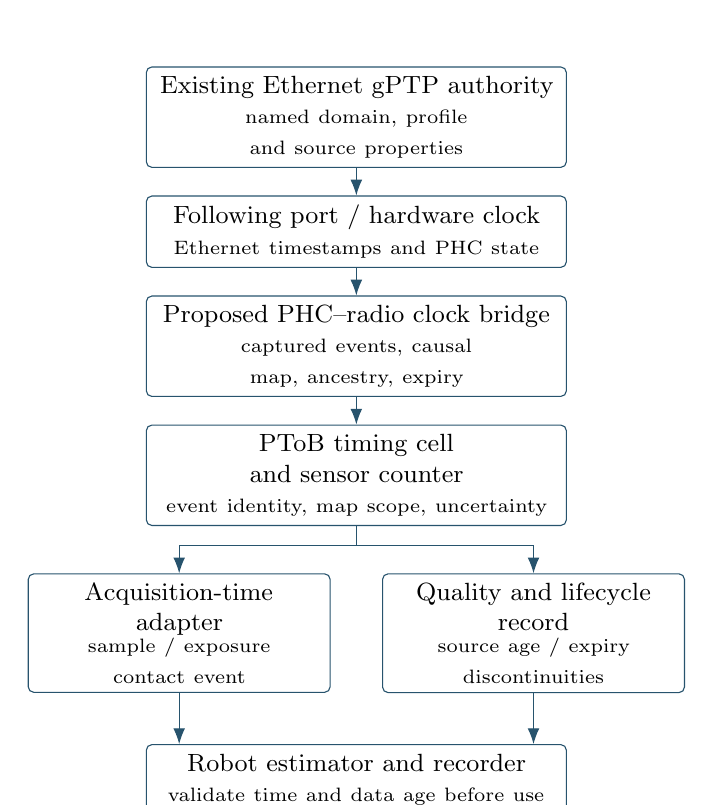
\begin{tikzpicture}[font=\small,box/.style={draw=studyblue,rounded corners=2pt,align=center,minimum height=0.7cm,text width=5.1cm},branch/.style={box,text width=3.6cm},arr/.style={-{Latex[length=2mm]},draw=studyblue}]
\node[box] (gm) {Existing Ethernet gPTP authority\\\scriptsize named domain, profile and source properties};
\node[box,below=0.35cm of gm] (phc) {Following port / hardware clock\\\scriptsize Ethernet timestamps and PHC state};
\node[box,below=0.35cm of phc] (bridge) {Proposed PHC--radio clock bridge\\\scriptsize captured events, causal map, ancestry, expiry};
\node[box,below=0.35cm of bridge] (ble) {PToB timing cell and sensor counter\\\scriptsize event identity, map scope, uncertainty};
\node[branch,below=0.6cm of ble,xshift=-2.25cm] (event) {Acquisition-time\\adapter\\\scriptsize sample / exposure\\contact event};
\node[branch,below=0.6cm of ble,xshift=2.25cm] (quality) {Quality and lifecycle\\record\\\scriptsize source age / expiry\\discontinuities};
\node[box,below=0.65cm of event,xshift=2.25cm] (robot) {Robot estimator and recorder\\\scriptsize validate time and data age before use};
\draw[arr] (gm)--(phc);\draw[arr] (phc)--(bridge);\draw[arr] (bridge)--(ble);
\draw[arr] (ble.south)--++(0,-0.25)-|(event.north);
\draw[arr] (ble.south)--++(0,-0.25)-|(quality.north);
\draw[arr] (event.south)--(robot.north -| event.south);\draw[arr] (quality.south)--(robot.north -| quality.south);
\end{tikzpicture}
\caption{Proposed Mode A dependencies. Ethernet TSN traffic and actuator control retain their own paths and acceptance criteria. The cross-clock bridge and robotics adapters are new work; the figure is not a demonstrated installation.}\label{fig:architecture}
\end{figure}

\subsection{Hardware association is the critical bridge}
Candidate associations include a PHC-generated periodic output captured by the radio MCU, a radio/MCU pulse captured by PHC external timestamping, or a hardware-supported cross-timestamp facility. Each route needs an identified electrical/reference event, counter units, capture quantization, fixed latency, asymmetry, drift, rollover and interrupt-loss treatment. A pulse train alone does not identify its integer second or source epoch; an associated descriptor must resolve that ambiguity. Transporting an identified capture record later is compatible with precise timing if the record's event and clock relationship are preserved.

Reading two clocks sequentially in userspace can bracket a relationship, but process scheduling and bus delays limit the justified interval. Selecting the fastest read does not establish a deterministic error bound. A bridge with only a USB or HCI arrival timestamp may be useful for a coarser service, provided that service retains the larger or unknown uncertainty. The critical artifact is a measured counter-to-PHC relationship, not the presence of Ethernet and Bluetooth on the same computer.

For a proposed single-board-computer gateway, an exact controller/driver capability inventory must establish support for the selected BLE timing path and PHC association. Bluetooth and Ethernet on the same board do not establish either capability. The macOS USB/chrony research is an application-clock extension, not an Ethernet PHC servo or gPTP bridge \cite{usb}. That earlier result cannot qualify either proposed bridge mode or relabel ordinary host time as measured PToB time.

\subsection{Keep clock control and graph direction unambiguous}
One process or controller owns adjustment of each physical clock. In Mode A, the Ethernet stack may discipline the PHC while a separate read/capture path estimates its relationship to the PToB counter; the estimator must not also drive that PHC from its BLE descendant. In Mode B, the admitted PToB source owns the output PHC discipline and the Ethernet stack's role is configured consistently. Switching modes requires an explicit lifecycle transition, not two simultaneous feedback loops.

An imported clock retains its original root ancestry. A bridge rejects a candidate source whose dependency graph contains that bridge or its downstream domain. PTP clock identity, PToB root identity and administrative authority are different namespaces; a configured binding relates them. The same upstream grandmaster appearing through two paths is one authority with correlated error, not two independent votes. Ethernet path information alone cannot reveal a loop hidden by a BLE conversion; the bridge needs a cross-protocol ancestry record.

\section{A proposed domain, event and quality contract}
Table~\ref{tab:contract} specifies semantics at the adapter boundary. It is not an implemented packet format. A future encoding can bind repeated fields to an immutable descriptor, but every event must identify that descriptor unambiguously through recording and replay.

\begin{table}[htbp]\centering\small
\caption{Minimum proposed robotics timing record. Unknown bounds remain unknown.}\label{tab:contract}
\begin{tabular}{@{}L{0.24\linewidth}L{0.70\linewidth}@{}}\toprule
Field group & Meaning and required scope\\\midrule
Coordinate and domain & Timescale/epoch, integer seconds plus exact fraction or ticks, range/era; administrative domain, PTP domain number and applicable profile/edition. Domain number alone is not a globally unique authority.\\\addlinespace
Source ancestry & Ethernet grandmaster identity and relevant time properties, PToB root/incarnation, bridge identity, selected ancestry and explicit cross-protocol bindings. Preserve origin age.\\\addlinespace
Clock map & Local boot/counter epoch, immutable map generation, rate/offset, causal publication time, valid interval and calibration identifier.\\\addlinespace
Physical event & Sensor and event identity, sequence, captured counter, acquisition definition and observation point; distinguish scheduled target from measured execution.\\\addlinespace
Quality and lifecycle & Tracking/holdover/expired/reacquiring state; source-observation age, validity deadline, uncertainty type, coverage assumptions, known bias and phase/frequency discontinuity record.\\\addlinespace
Application binding & Driver/message schema, configuration, frame/point/sample relation, data-age limit, queue deadline, consumer admission and replay/simulation state.\\\bottomrule
\end{tabular}
\end{table}

\subsection{Timescale correctness precedes precision}
A continuous domain coordinate, TAI, UTC, a POSIX-style system clock and ROS simulation time are not interchangeable. External UTC is not necessary for two sensors to share a local coordinate, but that local relationship must not be presented as civil-time traceability. Where a PTP-timescale domain and a UTC host are associated, Linux PTP documents the separate PHC and system-clock timescales and the need to maintain their offset \cite{phc2sys}. A whole-second association error dominates a nanosecond-scale fractional residual.

The proposed adapter records time properties and their validity and applies only verified conversions. It never infers a current UTC offset from a remembered constant or changes the meaning of an existing root epoch. TAI representation and time-property propagation would be explicit future firmware work; this paper does not claim that current PToB firmware implements them. A synthetic leap, unknown offset, source-epoch change and counter reset must all be tested without operating the robot.

\subsection{ROS 2 integration attaches time to acquisition}
ROS distinguishes SystemTime, SteadyTime and ROSTime; simulated ROS time can pause or jump and is activated through \code{use\_sim\_time} \cite{rosclock}. The proposed driver converts an identified acquisition counter through its qualified map before setting a sensor message timestamp. The official Image message definition requests acquisition time \cite{rosimage}; a callback's current time is not equivalent. For a rolling-shutter image or a scanning lidar, a single frame timestamp needs an explicit row/point timing model.

Existing message timestamps do not carry this paper's complete source-quality contract. A proposed companion record therefore binds quality, source generation and acquisition semantics to the same sensor event sequence. Association loss makes that event unqualified; receipt of a recent status message does not retroactively qualify every queued sample. Live deadlines and hardware timeouts use a monotonic basis, with conversion to the shared event coordinate at the boundary. Simulation/replay time is fenced from live actuation, and recorded original timestamps remain distinguishable from replay scheduling time.

\section{Causal clock composition and the error budget}\label{sec:budget}
\subsection{Compose maps without using future information}
Let $c$ be an endpoint counter, $p$ a bridge PHC coordinate and $T$ the selected domain time. For an immutable generation, write
\begin{equation}
 \widehat p(c)=p_0+a(c-c_0),\qquad
 \widehat T(p)=T_0+b(p-p_0),\qquad
 \widehat T(c)=T_0+ba(c-c_0).
 \label{eq:compose}
\end{equation}
Here $a$ converts counter ticks to PHC units and $b$ converts PHC units to domain units. The simplification assumes matched anchors; general affine maps retain their explicit intercepts. Additional relay maps compose similarly but add validity and uncertainty dependencies. A generation is usable only within every constituent map's permitted interval, with matching source and counter scopes.

For online decisions, all map generations and calibration constants must be available before the decision deadline. An acquisition-time claim of causal mapping uses a map already available at acquisition; any later reconstruction is separately marked retrospective. Arrival of a delayed sample does not make an expired source current. A future output requires the validity and error model to cover its scheduled execution interval, not just its enqueue time. An acknowledgement establishes a software event unless an independent execution capture proves more.

\subsection{Do not turn residual RMS into a bound}
In common time units, a proposed end-to-end budget is
\begin{equation}
 E_{\rm event} \leq E_{\rm domain}+E_{\rm PHC\leftrightarrow radio}
 +E_{\rm BLE}+E_{\rm capture}+E_{\rm sensor}+E_{\rm conversion}.
 \label{eq:budget}
\end{equation}
The inequality is meaningful only when every term is a justified compatible bound over the stated operating envelope. A standard deviation, conditional RMS, calibration residual and guaranteed maximum are different quantities. Correlated source and fit errors do not justify root-sum-square aggregation. Unknown asymmetry, antenna/path delay, sensor latency or output delay leaves the end-to-end bound unknown. A measured finite maximum describes its population; it is not automatically a worst-case guarantee.

Pairwise sensor agreement has a different budget from absolute domain error. A common root error can cancel in a relative difference while distinct local path biases remain. Conversely, agreement between two descendants of one root cannot validate that root against UTC. Electrical trigger generation and actual sensing/actuation introduce their own terms after the shared clock. Calibration must bind to board, firmware, rate, sensor mode, path, temperature envelope and event definition, with independent validation data rather than a fitted offset reported as a test result.

\subsection{Finite holdover is a service contract}
For elapsed time $\tau$ since the last admissible observation, consider a hypothetical bound
\begin{equation}
 E(\tau)=E_0+\rho_{\max}\tau+\tfrac12\alpha_{\max}\tau^2,
 \label{eq:holdover}
\end{equation}
where $E_0$ is an initial error bound in seconds, $\rho_{\max}$ is a fractional-frequency bound and $\alpha_{\max}$ bounds its rate of change per second. This model is a proposal, not measured oscillator performance. Temperature, vibration, supply changes and estimator transients may invalidate an assumed bound.

With $E_0=0.2\us$, $\rho_{\max}=0.5\ppm$ and $\alpha_{\max}=0$, an assumed $10\us$ service expires after $19.6\,\mathrm{s}$; an assumed $1\us$ service expires after $1.6\,\mathrm{s}$. Adding $\alpha_{\max}=0.02\,\mathrm{ppm/s}$ reduces the first deadline to approximately $15.0625\,\mathrm{s}$. These examples show why one ``locked'' flag cannot serve every consumer. If a future scheduled event lies beyond the allowed interval, it is rejected even while current samples remain admissible. Firmware expiry and acquisition-gap policy may impose an earlier deadline.

\section{Shared time does not close a TSN or control deadline}
\subsection{Gate margin and nonpreemptive blocking}
Consider a deliberately simplified one-hop schedule. A packet is ready before a nominal window, an admitted scheduler chooses its position, and all quantities use the same nominal time coordinate. Let window width be $W$, frame serialization time $t_f$, maximum relative clock misalignment $\epsilon_{\rm rel}$, and a symmetric non-clock implementation margin $J$. A conservative containment condition for this toy model is
\begin{equation}
 W\geq t_f+2(\epsilon_{\rm rel}+J).
 \label{eq:window}
\end{equation}
The margin applies at both window boundaries. This is not the IEEE gate algorithm or a network schedulability theorem. Multi-hop forwarding, release jitter, link propagation, queue interference, guard bands, rate error and hardware gate behavior require their own constraints.

For an assumed total wire occupancy of 256 bytes including the framing/gap allowance selected for this example, $t_f=20.48\us$ at 100 Mbit/s and $2.048\us$ at 1 Gbit/s. With $W=50\us$, $\epsilon_{\rm rel}=1\us$ and $J=2\us$, Equation~\ref{eq:window} requires $26.48\us$ and leaves $23.52\us$ of nominal slack at 100 Mbit/s. Raising the assumed misalignment to $15\us$ requires $54.48\us$ and fails that window. Two clocks each bounded by $\pm1\us$ against a common coordinate generally require a $2\us$ pairwise bound unless correlation justifies less.

With preemption disabled, an already transmitting frame of an assumed 1542-byte total wire occupancy consumes $123.36\us$ at 100 Mbit/s, or $12.336\us$ at 1 Gbit/s. Priority alone cannot interrupt that frame. A guard interval or qualified preemption mechanism must account for blocking \cite{qbu}; residual fragments and overhead still matter when preemption is enabled. The small clock-fit residual of a BLE endpoint supplies none of these protections.

\subsection{A missed cycle can dominate an accurate timestamp}
Let an end-to-end deadline be $D$. A schematic requirement is
\begin{equation}
 L_{\rm acquisition}+L_{\rm release}+L_{\rm transport}
 +L_{\rm execution}+L_{\rm output}\leq D,
 \label{eq:deadline}
\end{equation}
with bounded terms over the admitted workload. Timestamp error is tracked alongside this latency budget. A correctly timestamped old sample can still be unusable. For a hypothetical 1 ms cycle and $D=0.5\ms$, missing a transmission window by $1\us$ can add nearly a full cycle and violate the deadline even with a $100\ns$ clock error.

Wireless payload delivery therefore has an explicit age/deadline policy distinct from the timing broadcast. The first pilot uses PToB for acquisition-time association and preserves the existing wired actuator/control paths. Future command delivery needs bounded queueing, cancellation, sequence/replay protection, effective-time semantics and independently observed execution. Admission of a new clock source cannot substitute for a control-system timing analysis or any required functional-safety evidence.

\section{What existing PToB evidence supports}\label{sec:evidence}
Table~\ref{tab:evidence} preserves separate populations. The evidence motivates investigating event-associated clock transfer; it does not measure the proposed Ethernet-to-radio bridge or a robot endpoint. The values are conditional source-relative observations, not interchangeable bounds in Equation~\ref{eq:budget}.

\begin{table}[htbp]\centering\small
\caption{Selected historical observations, with their original missingness and endpoints. No cross-platform precision ranking or pooled result is inferred.}\label{tab:evidence}
\begin{tabular}{@{}L{0.19\linewidth}L{0.40\linewidth}L{0.34\linewidth}@{}}\toprule
Collection & Reported result and population & Limit for this adaptation\\\midrule
V14, 12 October & 436 usable relative PPS phase samples / 602 nominal opportunities; conditional RMS $62.504\ns$. Other categories: 65 invalid reference, 3 expired maps, 98 unobserved \cite{v14}. & The 501 all-causal samples have RMS $3.929\ms$. Fractional phase is not independent UTC, continuous availability or gPTP output.\\\addlinespace
S3, 22 October & Fixed 660 s attempt: 615 valid, 1 invalid, 44 unrecorded nominal opportunities; conditional RMS $110.801\ns$, maximum absolute residual $402\ns$ \cite{s3}. & Original attempt remains incomplete and failed. Collection disabled; final fence absent. RF endpoint and independent output accuracy remain unqualified.\\\addlinespace
USB, 17 October & Separate concurrent 180 s shared-bus RC/DC comparison with distinct RX, chrony and availability populations \cite{usb}. & Host application-clock agreement is not a NIC PHC transfer, a clean-bus experiment or a robotics acquisition result.\\\bottomrule
\end{tabular}
\end{table}

The S3 campaign's separate raw 80 MHz observer was off during its prospective PPS experiment. Digital activity observations do not by themselves identify an RF packet reference plane \cite{s3}. A numerical ratio between these historical RMS values and a TSN specification would mix population, endpoint, missingness and bound semantics. In particular, once-per-second phase observations cannot exclude subsecond excursions that matter to a cyclic controller.

The public derived records permit the stated offline recomputations while raw private captures and exact-device operational records remain excluded. Their publication does not grant access to hardware or promote any firmware into a robotics-qualified build. A new integration needs its own frozen source identities, instruments, calibration, independent observations and acceptance record.

\section{Loss, mobility and reconfiguration are part of the service}
\subsection{Quality is evaluated at the consumer's event}
The proposed lifecycle is unassociated, acquiring, tracking, bounded holdover, expired and reacquiring. These are semantic states for the adaptation, not a claim that current firmware exposes this exact API. Every consumer checks the original observation age, scope and uncertainty against its own service limit. Forwarding a fresh packet does not refresh an old upstream reference. A successful packet decode after an outage is not sufficient evidence of reacquired precision.

On expiry, pending qualified outputs are cancelled or rejected where the endpoint can enforce that policy. Recorded samples may still be retained with degraded/unknown quality for offline analysis. A sensor that free-runs after source loss needs an observable state and a qualified local holdover model. If the endpoint cannot expose invalidity, the integration must disclose that loss and avoid representing its outputs as continuously qualified.

\subsection{Root changes, tools and roaming require new scope}
A grandmaster change, administrative domain transition, PToB root incarnation change, local reboot, counter wrap ambiguity or calibration change fences old maps and queued decisions. Continuous numerical time across a handover is not proof of a continuous error bound. A proposed handover record includes the old/new authorities, detected discontinuity, admission interval, map generations and first independently qualified event after reacquisition.

For roaming between robot cells, simultaneous reception of two roots does not prove that their times are comparable. A measured inter-domain relationship or a fresh association is required. Metal structures, orientation changes, people, nearby radios and radio coexistence are test variables. Faster movement can change propagation and receive geometry; any assumed fixed path correction must survive the specified envelope. Topology depth and relay counts are experimental factors, not supported limits inferred from a timing fit.

\subsection{Authentication and independence have limited meanings}
PToB group authentication can support membership and freshness under its threat model; it does not establish physical source correctness, eliminate delay attacks, or preserve authenticity through an unrelated Ethernet profile. A signed or authenticated descriptor still needs a justified event association. A gateway that translates identities must make that trust boundary visible. Redundant transport paths and multiple receivers sharing one authority must not be counted as independent metrological references. Failure analysis records common-mode dependencies explicitly.

\section{A staged and falsifiable validation programme}\label{sec:validation}
\subsection{Gate 0: freeze the service and reproduce offline}
Choose Mode A first, one named Ethernet domain, one PHC/radio platform, one sensor event and one application. Specify the target event-error limit, data-age limit, permitted temperature/load/topology envelope, required valid fraction, maximum gap and recovery criterion before collecting data. Freeze source versions, profile/edition, configuration, instrument calibration and counter definitions. A profile-conformance matrix remains separate from an application acceptance matrix.

Offline checks cover map composition and inverse consistency, causal publication fences, interval intersection, rollover/reset, epoch and synthetic leap conversions, unknown-bound propagation, holdover expiry and queued-event rejection. Replay synthetic ROS time pauses and backwards jumps without a live actuation path. The included analytical verifier checks this paper's examples and edition identity; it implements neither gPTP nor a robot controller.

\subsection{Gate 1: establish a wired timing baseline}
Use a separately scoped testbed with a named gPTP source, following PHC and identified measurement outputs. Verify the exact profile/media and port eligibility, source/time properties, clock-control ownership and physical timestamp reference planes. Independently measure source-to-PHC phase/frequency and lifecycle under link loss, grandmaster replacement, load and restart. Preserve all loss and reacquisition intervals. A servo's own offset log is diagnostic evidence; it cannot be its only independent accuracy witness.

\subsection{Gate 2: isolate and measure the cross-clock bridge}
Characterize the PHC-to-radio relationship before adding a BLE receiver. Capture corresponding identified events with an independently characterized time-interval instrument or capture system. Include pulse integer-second association, direction-dependent delay, cable/pin latency, drift, temperature, buffering, missed captures and counter wrap. Keep calibration and held-out validation separate. Reject the route if its demonstrated uncertainty consumes the service budget or if its physical event cannot be identified.

\subsection{Gate 3: qualify one wireless acquisition path}
Add one PToB endpoint and a simple sensor event. Compare hardware acquisition timestamps with an independently observed stimulus shared with a wired reference. For an IMU, an electrical data-ready edge alone characterizes interface timing unless the internal sampling aperture is also established. A camera test measures exposure timing rather than just the returned image timestamp. Record per-event residuals, validity, sequence, map generation and data arrival age. Increase duration and stress only after the basic event association is correct.

Controls compare the same sensor/interface under its local clock, a wired reference where available, and the PToB extension, with the same stimulus and analysis. They do not compare unrelated published RMS values. Predeclare no-retuning validation windows. Include cold start, power cycle, source withdrawal, RF obstruction/interference, CPU/transport load, thermal change and relay/topology factors. No observer path may feed the estimator being evaluated.

\subsection{Gate 4: bounded robotics fusion pilot}
Integrate the validated sensor driver and quality record with one estimator/recorder while retaining qualified wired control. Independently measure the shared physical event, then evaluate timestamp use, queue age, drop/reject behavior, estimator consistency and a predefined spatial/task outcome. Inject delayed payloads with correct timestamps as well as incorrect epochs, stale quality, duplicate events, source changes and ROS replay transitions. This distinguishes a useful sensor-time service from a pipeline that merely displays a synchronized clock.

One candidate preregistration is a 30-minute baseline at an assumed 1 kHz acquisition rate: $1{,}800{,}000$ nominal opportunities. For discussion, set an event-time objective of $10\us$, a qualified fraction of at least 99.9\%, a maximum unqualified acquisition gap of $20\ms$, and a maximum accepted data age of $20\ms$. This requires at least $1{,}798{,}200$ qualified opportunities and permits at most 1800 unqualified opportunities; the total allowance cannot hide a long contiguous outage. These are proposed pilot choices, not robotics-wide requirements, current PToB capabilities or a motion-control authorization.

For this candidate record, an event counts as qualified only if its source and map are admissible, its physical acquisition is independently associated, and its absolute measured residual plus justified measurement uncertainty is at most $10\us$. If that uncertainty is unavailable, the opportunity cannot pass. Report every admitted event exceeding the threshold as a timing violation and retain it in the admitted-event residual distribution; do not censor it from the error statistics. The receiver rejects over-age data and wrong-scope events rather than accepting a plausible timestamp. Report cold-start behavior separately from the predeclared baseline start; report every deliberate fault window and its missingness in additional predeclared populations. Do not remove unexpected outages from the baseline after observing them. Reacquisition passes only after the independent event criterion is restored. A finite pass establishes this campaign's observed outcome and does not prove a deterministic bound.

\subsection{Gate 5: optional Ethernet egress and scheduled output}
Only after the preceding gates, evaluate Mode B on an isolated island with its own admitted PHC control and profile implementation. Verify source quality and traceability translation, selection behavior, eligibility, packet interoperability and output timing through expiry/recovery. Separately measure any scheduled output or actuator response with independent instrumentation, including missed windows, overruns, cancellation and discontinuities. Functional interoperability, standards conformance, timing acceptance and any functional-safety qualification are distinct outcomes.

\subsection{Count missing opportunities and clustered failures}
For a predeclared window, let $N_{\rm expected}$ be the stated nominal opportunity count. Partition its opportunities as
\begin{equation}
 N_{\rm expected}=N_{\rm qualified}+N_{\rm invalid}
 +N_{\rm expired}+N_{\rm missing}.
 \label{eq:counts}
\end{equation}
Define mutually exclusive classification precedence in advance, for example invalid before expired; transport duplicates are reported separately. Distinguish nominal opportunities from independently counted physical events. Report qualified fraction, missing and degraded intervals, maximum gap, cold-start/recovery duration, signed bias, uncentered RMS, specified quantiles, finite maxima and uncertainty at the named physical endpoint. A conditional histogram never replaces the opportunity denominator. State results both within and outside the admitted envelope.

As an illustrative statistical limit, zero observed violations in $N$ independent Bernoulli trials gives a one-sided 95\% upper violation probability $1-0.05^{1/N}$. At $N=10^6$, this is approximately $2.996\times10^{-6}$ per trial. At 1 kHz, that population lasts only 1000 s. Actual clock/control errors can be strongly correlated, so that calculation does not establish a reliability or safety claim; outage clusters, long-term drift and systematic failures need separate analysis. A finite campaign cannot prove a deterministic bound by absence of observed violations.

\section{Implementation priorities and research decision}
The first deliverable should be a read-only time/quality interface from an existing synchronized PHC, one hardware-associated radio map, and one acquisition-time adapter. Those modules expose the uncertain boundary directly and support replay without operating devices. Versioned semantic records and source ancestry come before a generalized multi-vendor gateway. One measured sensor integration is more informative than a broad list of nominal PTP/BLE capabilities.

The next work item depends on the dominant budget term. If cross-clock transfer dominates, change the capture path or target hardware. If sensor aperture uncertainty dominates, improve the device interface or reduce the claimed service. If payload age dominates, improve transport/admission rather than the clock fit. If roaming cannot preserve a valid source relationship, record an outage and reacquire. A design that works for an instrumented tool need not support synchronized joint actuation.

No energy saving, bill-of-materials advantage, replacement of existing industrial networks, supported robot count or safe hop depth is established. Battery operation, radio/controller support, concurrent links, installation geometry, calibration and maintenance add costs that must be measured. The proposal succeeds only if the qualified extension improves the chosen robotics outcome while making outages and uncertainty inspectable. Failure to meet an acquisition or lifecycle gate is a useful negative result, even if the radio clock's conditional residual remains small.

\section{Conclusion}
PToB is a plausible research path for extending a named robotic gPTP time domain to wireless acquisition endpoints. The defensible initial architecture follows the wired authority, measures the PHC-to-radio relationship, preserves source/domain/event semantics and rejects stale or unbounded time at the consumer. Current standards and official interfaces offer integration routes, but neither shared timestamps nor historical BLE phase observations establish TSN scheduling, gPTP conformance or physical robot synchronization. A qualified single-sensor path with independent event evidence is the next testable claim. Ethernet egress, roaming continuity and scheduled actuation remain later, separately measured extensions.

\appendix
\section{Reproduction and edition identity}
The standalone LaTeX source embeds its bibliography and original vector figure. Publicly obtainable Tectonic can typeset it without a private checkout, device or vendor SDK:
\begin{verbatim}
mkdir -p artifacts/papers
tectonic --outdir artifacts/papers \
  papers/ptob-gptp-tsn-robotics-preprint.tex
python3 tools/verify_robotics_paper.py
\end{verbatim}
The edition receipt \path{papers/editions/gptp-tsn-robotics-2026-10-22.json} records source/PDF/verifier identity, cited local records, primary-source retrieval scope, compiler and rendered-page review. Engines and bundles can change PDF bytes and pagination; rebuilding does not silently replace the reviewed edition. Hashes establish identity, not accuracy. Existing historical receipts remain unchanged.

The offline verifier checks map composition and validity, explicit unknown bounds, motion and holdover examples, the simplified window and serialization budgets, binomial illustration, evidence denominators, citation keys and recorded hashes. Separate public collection tools reproduce the V14, S3 and USB summaries. These computations do not recreate the original raw acquisition, calibrate the instruments or operate hardware. No new experimental dataset is introduced.

\section{Proposed acceptance record}
For each future integration, record domain/profile/standard editions and amendments; source authority and cross-protocol ancestry; exact bridge, sensor, driver, firmware and configuration; clock-control owner; counter/epoch and physical-event definitions; calibration and independent-witness method; uncertainty type and operating envelope; data-age/deadline and expiry policy; every denominator, missing interval and failure; source changes and recovery; raw/derived rights and reproducible analysis. Record interoperability, conformance, application timing and remaining unknowns separately.

\clearpage
\begin{samepage}
\section*{Acknowledgements and disclosure}
The author acknowledges OpenAI Codex assistance with research organization, drafting and verification; responsibility for the claims remains with Jonathan Yantis. Named standards, software and products identify cited systems without implying endorsement or interoperability approval. The original figure is a proposed architecture, not a measurement trace. This locally prepared manuscript remains a research draft; no submission, public-review promotion or hardware authorization is implied.
\end{samepage}

\begin{thebibliography}{99}\small
\bibitem{viability} J. Yantis, \emph{PToB Viability: Rooted BLE Timing Meshes for Heterogeneous Edge Networks}, research draft, 16 October 2026. \path{papers/ptob-viability-preprint.tex}. \url{https://github.com/yantisj2/PToB}. Historical synthesis; PTP ingress proposed.
\bibitem{timecode} J. Yantis, \emph{A Shared Time Base for Bluetooth Timecode Ecosystems: PToB Architecture, Compatibility Boundaries, and a Validation Programme}, research draft, 22 October 2026. \path{papers/ptob-bluetooth-timecode-preprint.tex}. Architectural companion; no robotics integration evidence.
\bibitem{modular} C. San Vicente Guti\'errez et al., ``Time Synchronization in modular collaborative robots,'' arXiv:1809.07295v1, 2018, especially Section III and its timestamp endpoints. \url{https://arxiv.org/html/1809.07295v1}. Accessed 22 October 2026. Historical experimental setup, not a current ROS guarantee.
\bibitem{robottsn} C. San Vicente Guti\'errez et al., ``Time-Sensitive Networking for robotics,'' arXiv:1804.07643v2, 2018, especially Section IV. \url{https://arxiv.org/html/1804.07643v2}. Accessed 22 October 2026. Original Ethernet shaping experiment; no BLE comparison.
\bibitem{as2025} IEEE SA, \emph{IEEE 802.1AS-2025: Timing and Synchronization for Time-Sensitive Applications}, official status and scope. \url{https://standards.ieee.org/ieee/802.1AS/11968/}. Accessed 22 October 2026. Published 17 December 2025; full normative text and amendment requirements not audited here.
\bibitem{industrial} IEEE 802.1, ``IEC/IEEE 60802 TSN Profile for Industrial Automation,'' official project status/scope; published IEC/IEEE 60802-2026, 29 June 2026. \url{https://1.ieee802.org/tsn/iec-ieee-60802/}. Accessed 22 October 2026. Profile scope/status, not normative clause inspection.
\bibitem{qbv} IEEE 802.1, ``802.1Qbv: Enhancements for Scheduled Traffic,'' project scope. \url{https://www.ieee802.org/1/pages/802.1bv.html}. Accessed 22 October 2026. Mechanism background; applicable consolidated edition must be selected.
\bibitem{qbu} IEEE 802.1, ``802.1Qbu: Frame Preemption,'' project scope and link-partner capability condition. \url{https://www.ieee802.org/1/pages/802.1bu.html}. Accessed 22 October 2026.
\bibitem{qci} IEEE 802.1, ``P802.1Qci: Per-Stream Filtering and Policing,'' project scope. \url{https://1.ieee802.org/tsn/802-1qci/}. Accessed 22 October 2026.
\bibitem{qcc} IEEE 802.1, ``P802.1Qcc: Stream Reservation Protocol (SRP) Enhancements and Performance Improvements,'' project scope. \url{https://1.ieee802.org/tsn/802-1qcc/}. Accessed 22 October 2026.
\bibitem{cb} IEEE 802.1, ``P802.1CB: Frame Replication and Elimination for Reliability,'' project scope. \url{https://1.ieee802.org/tsn/802-1cb/}. Accessed 22 October 2026.
\bibitem{ptp4l} Linux PTP Project, \emph{ptp4l(8)}, official manual, hardware/software timestamping, clock roles and \code{asCapable}. \url{https://www.linuxptp.org/documentation/ptp4l/}. Accessed 22 October 2026. Deployment version must be pinned separately.
\bibitem{gptpconfig} Linux PTP Project, ``gPTP,'' official example configuration. \url{https://www.linuxptp.org/documentation/configs/gptp/}. Accessed 22 October 2026. Example, not 802.1AS-2025/60802 certification.
\bibitem{phc} Linux Kernel, ``PTP hardware clock infrastructure for Linux,'' operations and optional ancillary features. \url{https://docs.kernel.org/driver-api/ptp.html}. Accessed 22 October 2026.
\bibitem{timestamping} Linux Kernel, ``Timestamping,'' hardware/software socket timestamp semantics. \url{https://cdn.kernel.org/doc/html/latest/networking/timestamping.html}. Accessed 22 October 2026. Driver and kernel version remain implementation-specific.
\bibitem{phc2sys} Linux PTP Project, \emph{phc2sys(8)}, ``Time Scale Usage.'' \url{https://www.linuxptp.org/documentation/phc2sys/}. Accessed 22 October 2026. Separate PHC/system-clock timescales; no daemon started for this study.
\bibitem{rosclock} T. Foote / ROS 2, ``Clock and Time,'' design documentation. \url{https://design.ros2.org/articles/clock_and_time.html}. Accessed 22 October 2026. Clock abstraction and simulation semantics, not timing qualification.
\bibitem{rosimage} ROS 2, \code{sensor\_msgs/msg/Image.msg}, official rolling-branch source, acquisition-time header comment. \url{https://raw.githubusercontent.com/ros2/common_interfaces/rolling/sensor_msgs/msg/Image.msg}. Accessed 22 October 2026; mutable branch. Rendered documentation access was restricted; original message source inspected.
\bibitem{basler} Basler, ``Precision Time Protocol,'' official product documentation, IEEE 1588-2008 and model-specific delay mechanisms/features. \url{https://docs.baslerweb.com/precision-time-protocol}. Accessed 22 October 2026. Documentation page carries a draft-version banner; no exact camera/firmware qualification or gPTP compatibility inferred.
\bibitem{v14} J. Yantis, V14 selected public evidence, 12 October 2026. \path{evidence/v14/2026-10-12/README.md}; \path{evidence/v14/2026-10-12/summary.json}. \url{https://github.com/yantisj2/PToB}. Distinct conditional/all-causal populations and nominal opportunity accounting.
\bibitem{s3} J. Yantis, \emph{Precision Bluetooth Timing on ESP32-S3: Causal Clock Discipline and Hardware Event Capture}, research draft and selected evidence, 22 October 2026. \path{papers/ptob-esp32s3-timing-preprint.tex}; \path{evidence/s3/2026-10-22/README.md}; \path{evidence/s3/2026-10-22/results.json}. Incomplete original 660-second attempt preserved.
\bibitem{usb} J. Yantis, \emph{Beyond USB Packet Arrival: Frame-Identified Time Transfer to macOS}, research draft, 17 October 2026. \path{papers/usb-macos-time-transfer-preprint.tex}; \path{evidence/usb/2026-10-17/README.md}. Fixed concurrent shared-bus 180-second comparison; metrics and withheld samples remain separate.
\end{thebibliography}
\end{document}
